\documentclass[11pt]{article}

% Insert style guide
\usepackage{my_thesis}
% Specifiy the location of images to be used
\graphicspath{{figures/}}

\begin{document}
\title{\textsc{Plasma based Structured Illumination Microscopy}\\}
\date{\footnote{Last Modified: \currenttime, \today.}}
\maketitle


\section{Abstract}
%
We present a linear high-resolution imaging scheme based on the plasma waves originating in the channel of field-effect transistors. The extremely small plasmonic wavelength along with a tunable illumination pattern in the far infrared region can resolve nano-scale objects over a broad range of frequencies.
%
\section{Introduction}
%
The resolution of a conventional fluorescent microscope is governed by the Abbe diffraction limit, restricting it to half the wavelength of the source used for illumination \cite{0521639212}. There are techniques that yield resolution beyond the diffraction limit, among them the most common is confocal microscopy, which uses pinholes to generate a focused point illumination and subsequently a high resolution image of the fluorescent sample. Despite improved resolution, the pinhole discards a portion of the emitted light due to which the signal level may become unusably low, particularly for weakly fluorescent biological samples. Moreover, because the point source illuminates only a small portion of the sample, it must be mechanically moved in order to scan the whole sample, therefore resulting in a slow imaging process. Structured Illumination microscopy (SIM) is a fast and wide-field microscopic technique in which the sample is illuminated by a non-uniform, modulated and spatially structured pattern revealing the high resolution information of a sample in the form of Moiré fringes \cite{Gustafsson_2000,Heintzmann1999a}. In order to yield a high resolution result, post-processing of a series of such images is performed to extract the high frequency content. A two-fold resolution enhancement is possible using linear SIM techniques. On the other hand, theoretically unlimited resolution enhancement can be obtained using non-linear techniques \cite{Gustafsson_2005}. However, such methods require very high intensities to illuminate the sample, increasing the likelihood of damage particularly in biological applications.

The idea of illuminating the sample with surface waves having wavelength much smaller than free-space wavelength at the same frequency was first proposed in \cite{Nassenstein_1970} resulting in superresolution. Surface plasmons existing at a metal-dielectric interface were used to excite a sample at optical frequencies in \cite{Wei_2010}. Similarly, in the mid-infrared frequency region, using graphene plasmons was proposed to achieve resolution two orders of magnitude beyond  the diffraction limit \cite{Zeng_2014}.

Plasma waves originating in the two-dimensional electron channel of field-effect transistors, discovered more than 30 years ago have lately received interest because of the potential to realize terahertz frequency sources and sensors \cite{Dyakonov_1993,Dyakonov_1996,Popov_2008,Otsuji_2006,Muravjov_2010}. The channel is formed at the interface of two semiconductor heterostructures in the shape of a two-dimensional electron gas (2DEG) and behaves as a plasma fluid with very high surface carrier density. For micron order lengths, the channel becomes a plasma cavity where the resonant frequency lies in the far-infrared (terahertz) frequency region and remarkably, can be tuned by varying the gate voltage. The gate bias also controls the electron velocity in the channel ranging from $.1 - 10 \times 10^6 m/s$ \cite{Burke_2000}. The 2DEG mobility below liquid nitrogen temperature (77 K) is very high $\approx 10^4 cm^2 V^{−1} s^{−1}$ \cite{Muravjov_2010}, resulting in undamped and low loss oscillations in the channel. It must be mentioned that substantial loss is introduced at room temperature because the mobility drops by at least two orders than the one listed above.

In this paper, we propose an extended structured illumination microscopy using plasma waves as the illumination source.

\section{Generating Illumination pattern}

Two-dimensional electron channels founA two-dimensional electron gas (2DEG) is an extremely thin region with a high concentration of electrons that are free to move along the interface of the semiconductor hetero-junctions found in field-effect transistors, leading to ballistic transport of electrons owing to high mobility.

Yahan ye batana ha ke 2deg surface waves support kerti ha. kaisay batana ha yeh nahi pata.

Aik tareeqa to yeh ha ke ap ye keh do ke since the 2DEG can be considered a sheet of charge sandwiched between dieelctric media, it supports surface waves. the conductivity is given as:
%
\begin{equation}
  \sigma_s(\O) = \frac{N_s e^2 \tau_{p}}{m^{\ast}}\frac{1}{1 + j \O \tau_{p}}
  \label{eq:conductivity}
\end{equation}
%
Neglecting any scattering effects in the 2DEG, the dispersion relation for plasma waves is expressed as \cite{Nakayama_1974}:
%
\begin{equation}
  \frac{\E_1}{k_{z1}} + \frac{\E_2}{k_{z2}} = -\frac{\sigma_s(\O)}{\O}
  \label{eq:disp_TM_two}
\end{equation}
%
where $\E_1$ and $\E_2$ are the dielectric constants of the barrier and substrate layers respectively and $k_{zi} = \sqrt{k_0^2 \E_i(\O) -  k_x^2}$ is the transverse propagation constant with $k_0$ being the free-space wavenumber.


When the source and drain terminals of the transistor are biased with a dc current source, the voltage buildup across the 2DEG creates an electron flow that is sinusoidal.
\begin{equation}
\end{equation}

\section{Imaging Technique}
%
The SIM technique can be split into two operations; one at the sample end and the other on the microscope end. First, the sample is illuminated with a non-uniform, modulated pattern of sinusoidal shape. Only the portion of the sample that falls under the peak of the illumination signal is focused while the rest of the sample remains unfocused. Other portions are focused by laterally shifting the illumination pattern. Through \emph{optical sectioning} of the sample, a number of acquired are combined to generate a focused
1. It creates optical sectioning that is excite different lateral portions of the sample by shifting of the pattern. The portion of the sample that is illuminated by the peak of the pattern is excited and it fluoresces while the rest of the sample is illuminated homogeneously by a uniform pattern. When the pattern is shifted, other portions of the sample are illuminated. This way the whole sample can be sequentially illuminated with high localized focused areas.

2. The other part of SIM deals with generation of Moiré effect that actually results in high resolution. The effect is created when the illumination signal is modulated by the sample signal
The objective lens of a microscope can be considered as a low-pass filter due to diffraction. The impulse response of the filter, i.e., the image of a point source, is a blurred spot termed as the \emph{point spread function}(PSF) of the microscope. When a sample that can be represented by $f(x,y)$ is illuminated by a signal $i(x,y)$, the output image, $m(x,y)$ of the microscope can be written in the spatial domain as \cite{Jost_2013}:
In terms of filter theory, the objective lens of a microscope can be considered as a diffraction limited low-pass filter that has a passband spanning up to $2k_0$ under ideal circumstances where $k_0$ is the free-space wavenumber. The impulse response of the filter, i.e., the image of a point source, is a blurred spot termed as the \emph{point spread function}(PSF) of the microscope. When a sample that can be represented by $f(x,y)$ is illuminated by a signal $i(x,y)$, the output image, $m(x,y)$ of the microscope can be written in the spatial domain as \cite{Jost_2013}:

%
where $\tau_p$ is the momentum relaxation time and $m^{\ast}$ is the effective  mass of electrons. When the


\begin{figure}[h!]
  \centering
  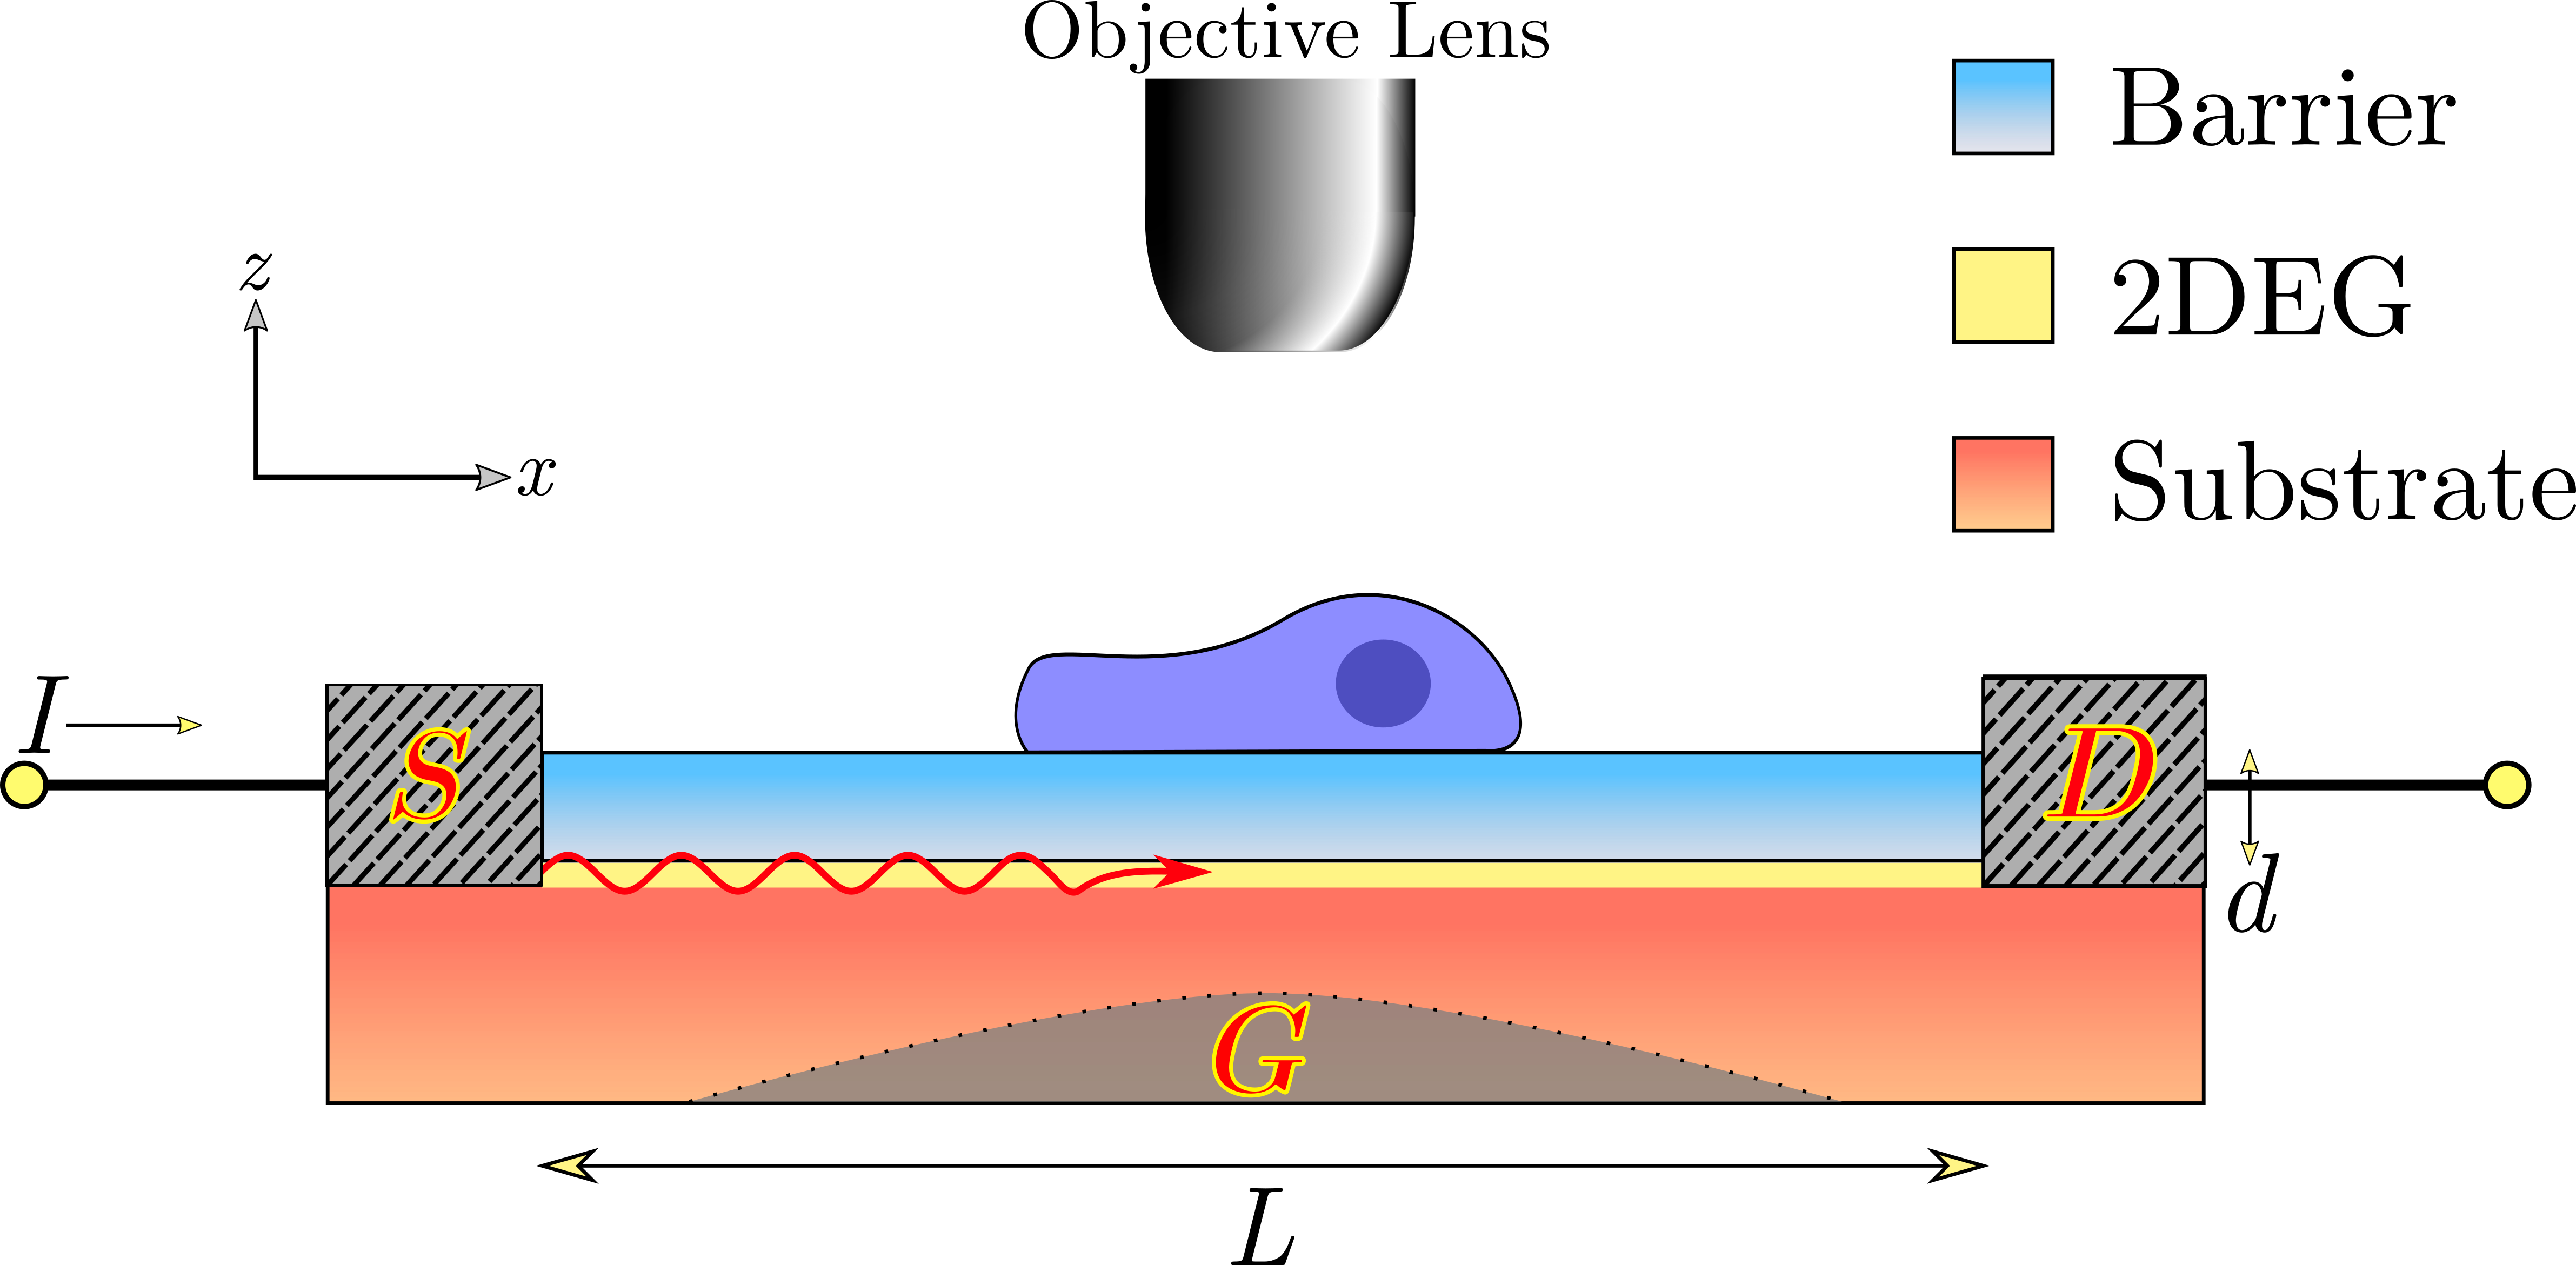
\includegraphics[scale=.5]{Microcopic_Structure.png}
  \caption{Schematic of the structure. 2DEG exists between a barrier layer of thickness $d$ and substrate}
  \label{fig:scheme}
\end{figure}

\begin{figure}[h!]
  \centering
  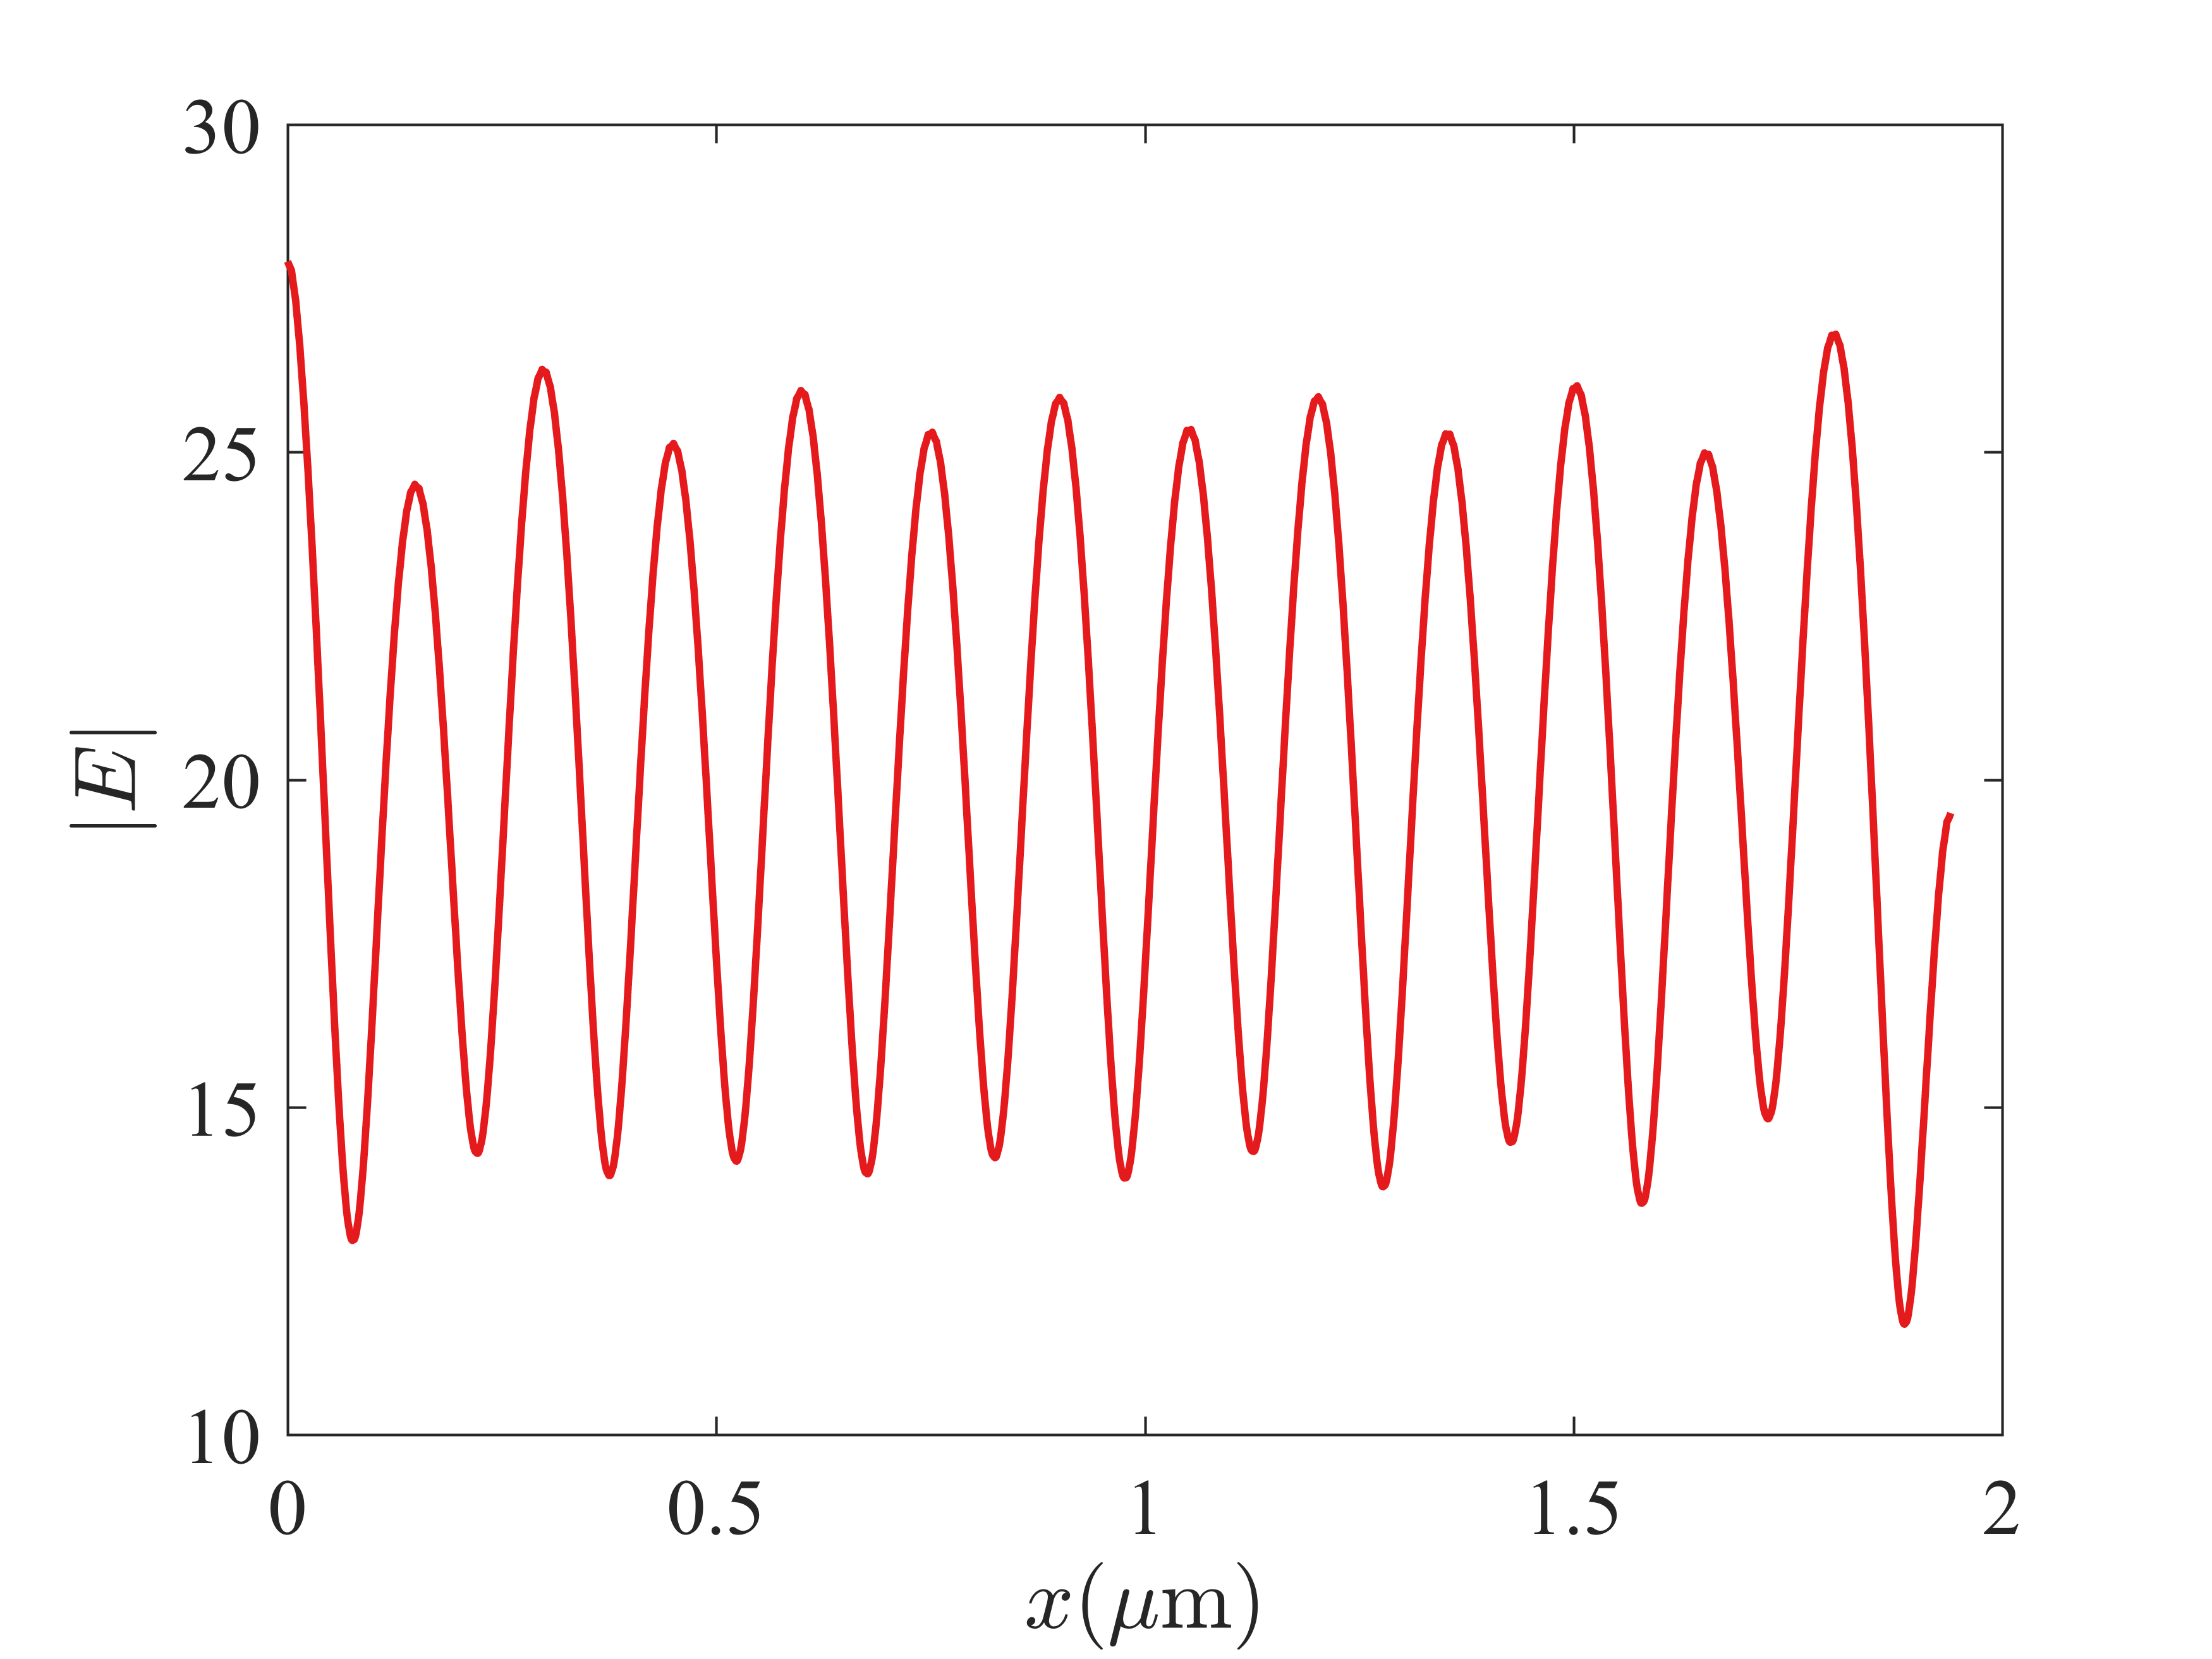
\includegraphics[scale=.5]{no_port.png}
  \caption{Absolute value of electric field along the $2 \u \mathrm{m} $ long channel GaAs/AlGaAs heterostructure}
  \label{fig:standing_wave}
\end{figure}

\begin{figure}[h!]
  \centering
  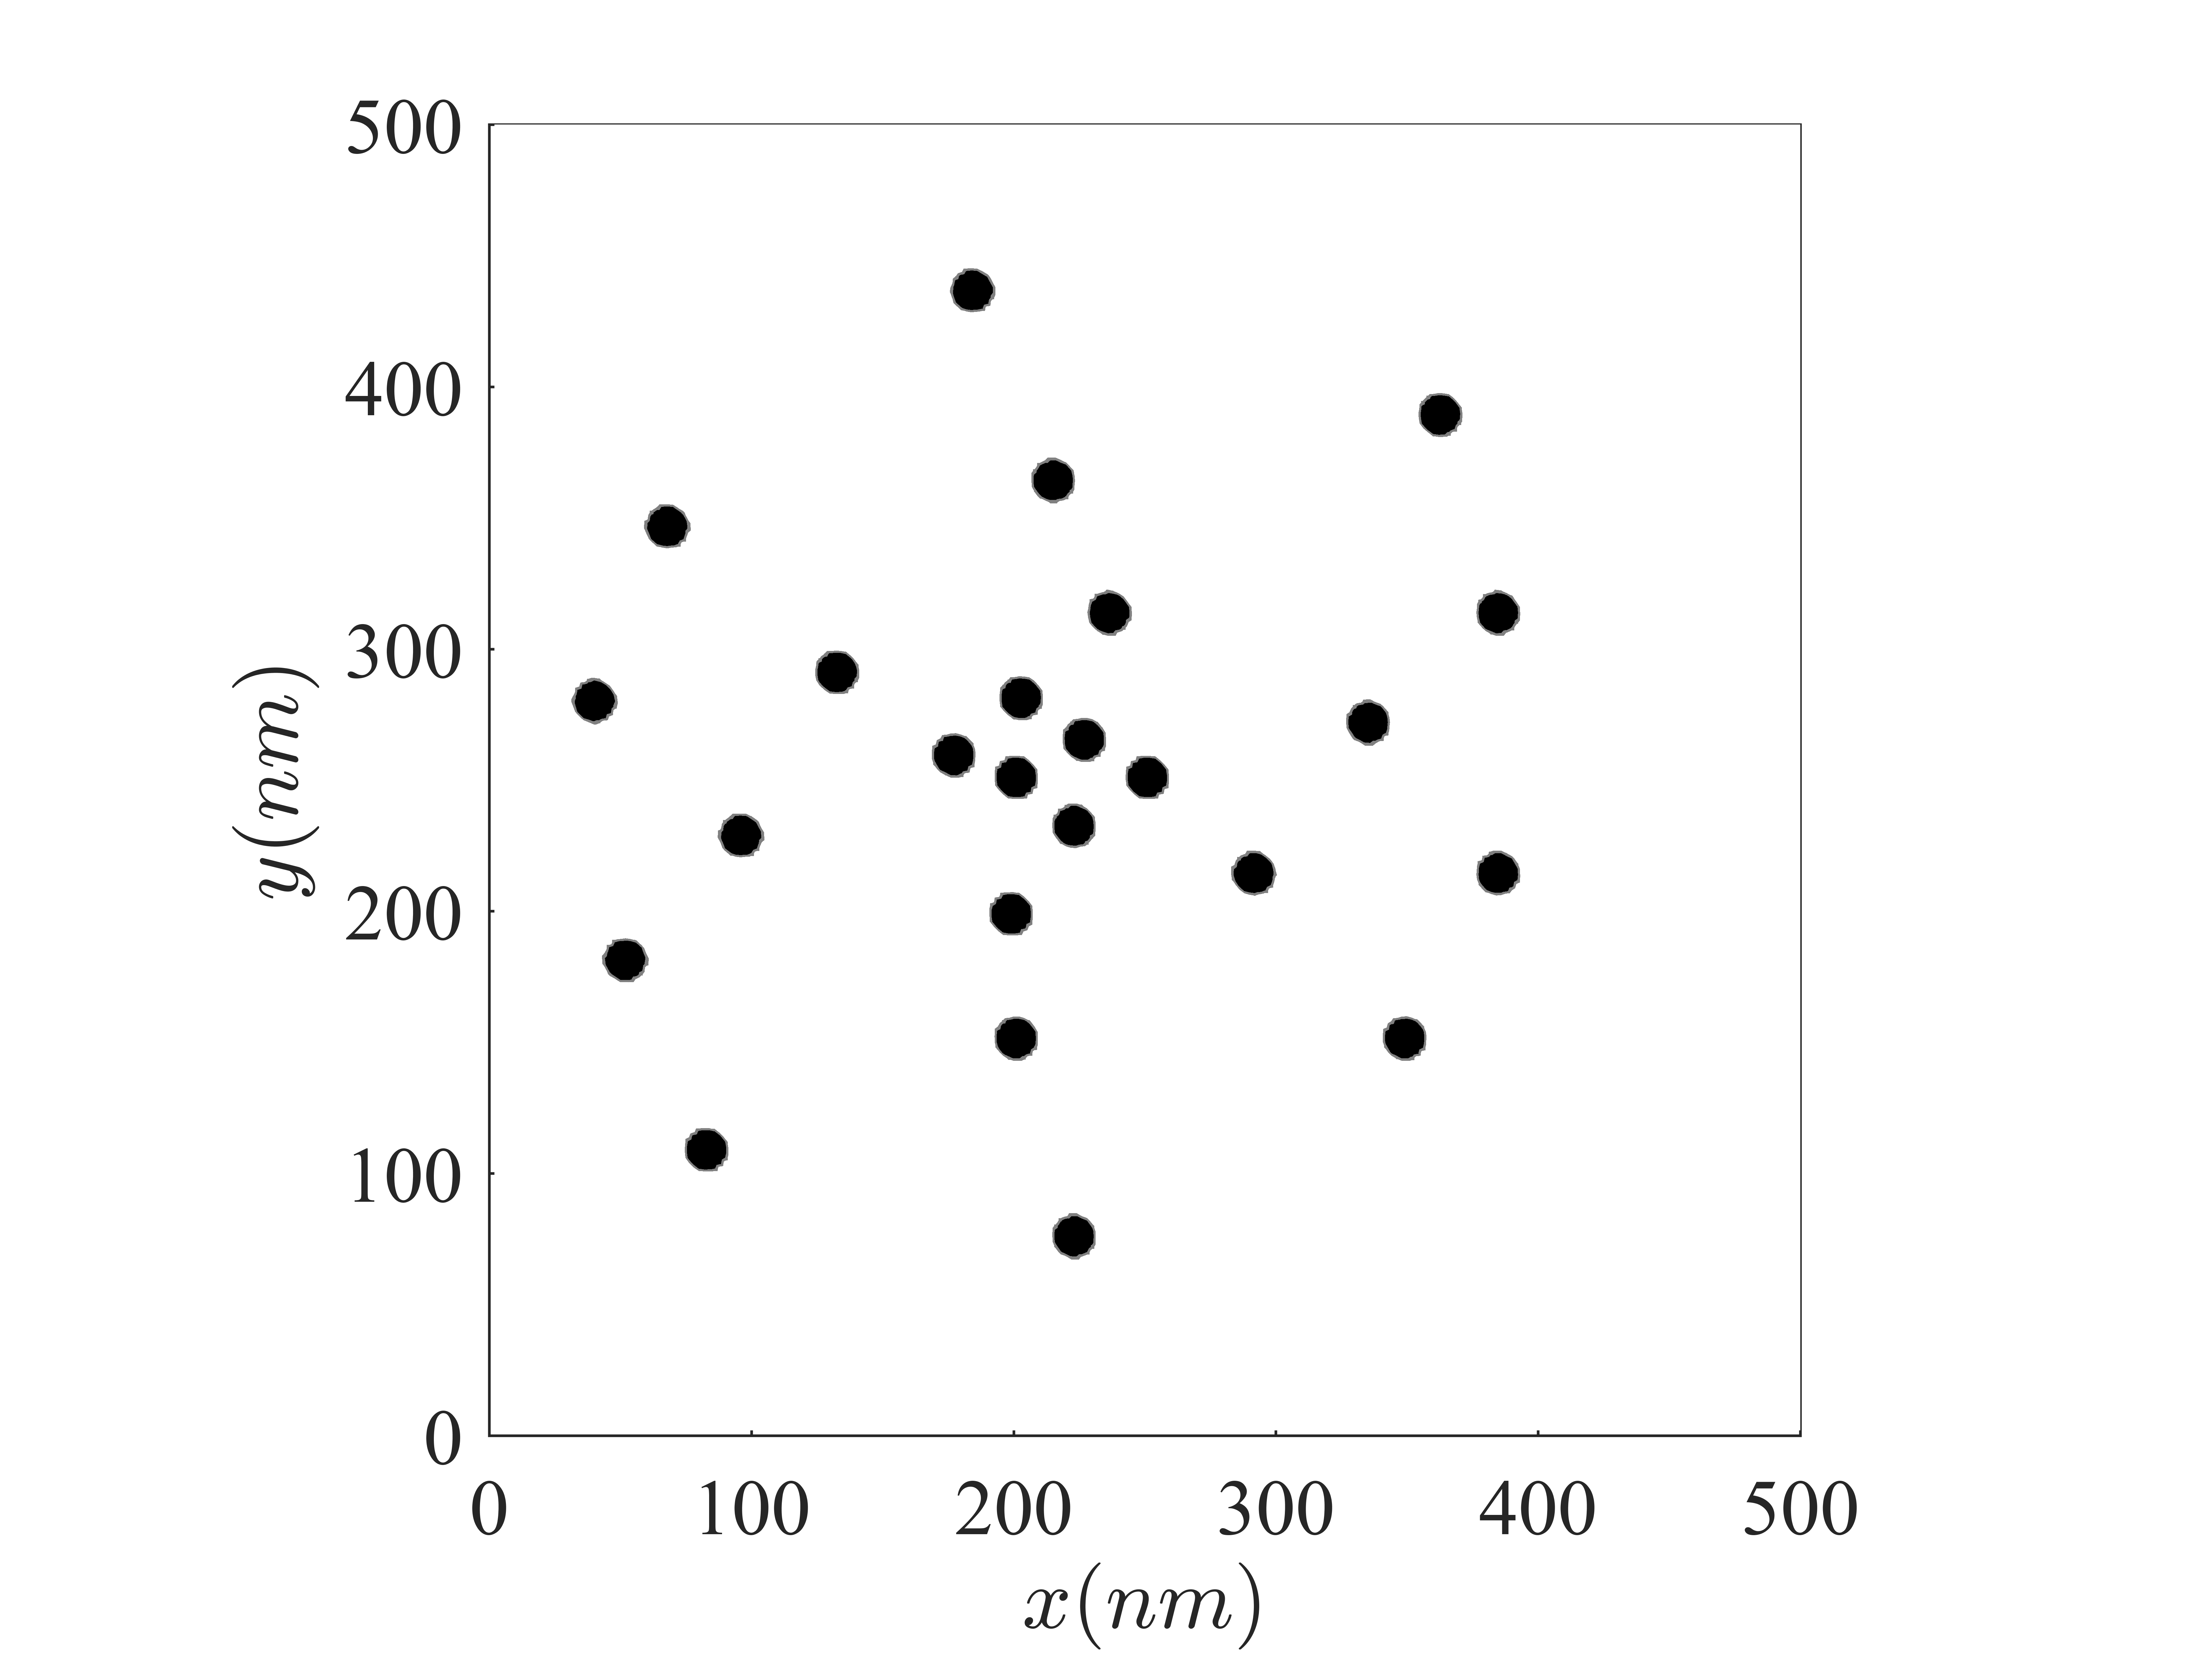
\includegraphics[scale=1]{test.png}
  \caption{Test image with $15$ nm fluorescent beads in a $500$ nm square space}
  \label{fig:scheme}
\end{figure}

\begin{figure}[h!]
  \centering
  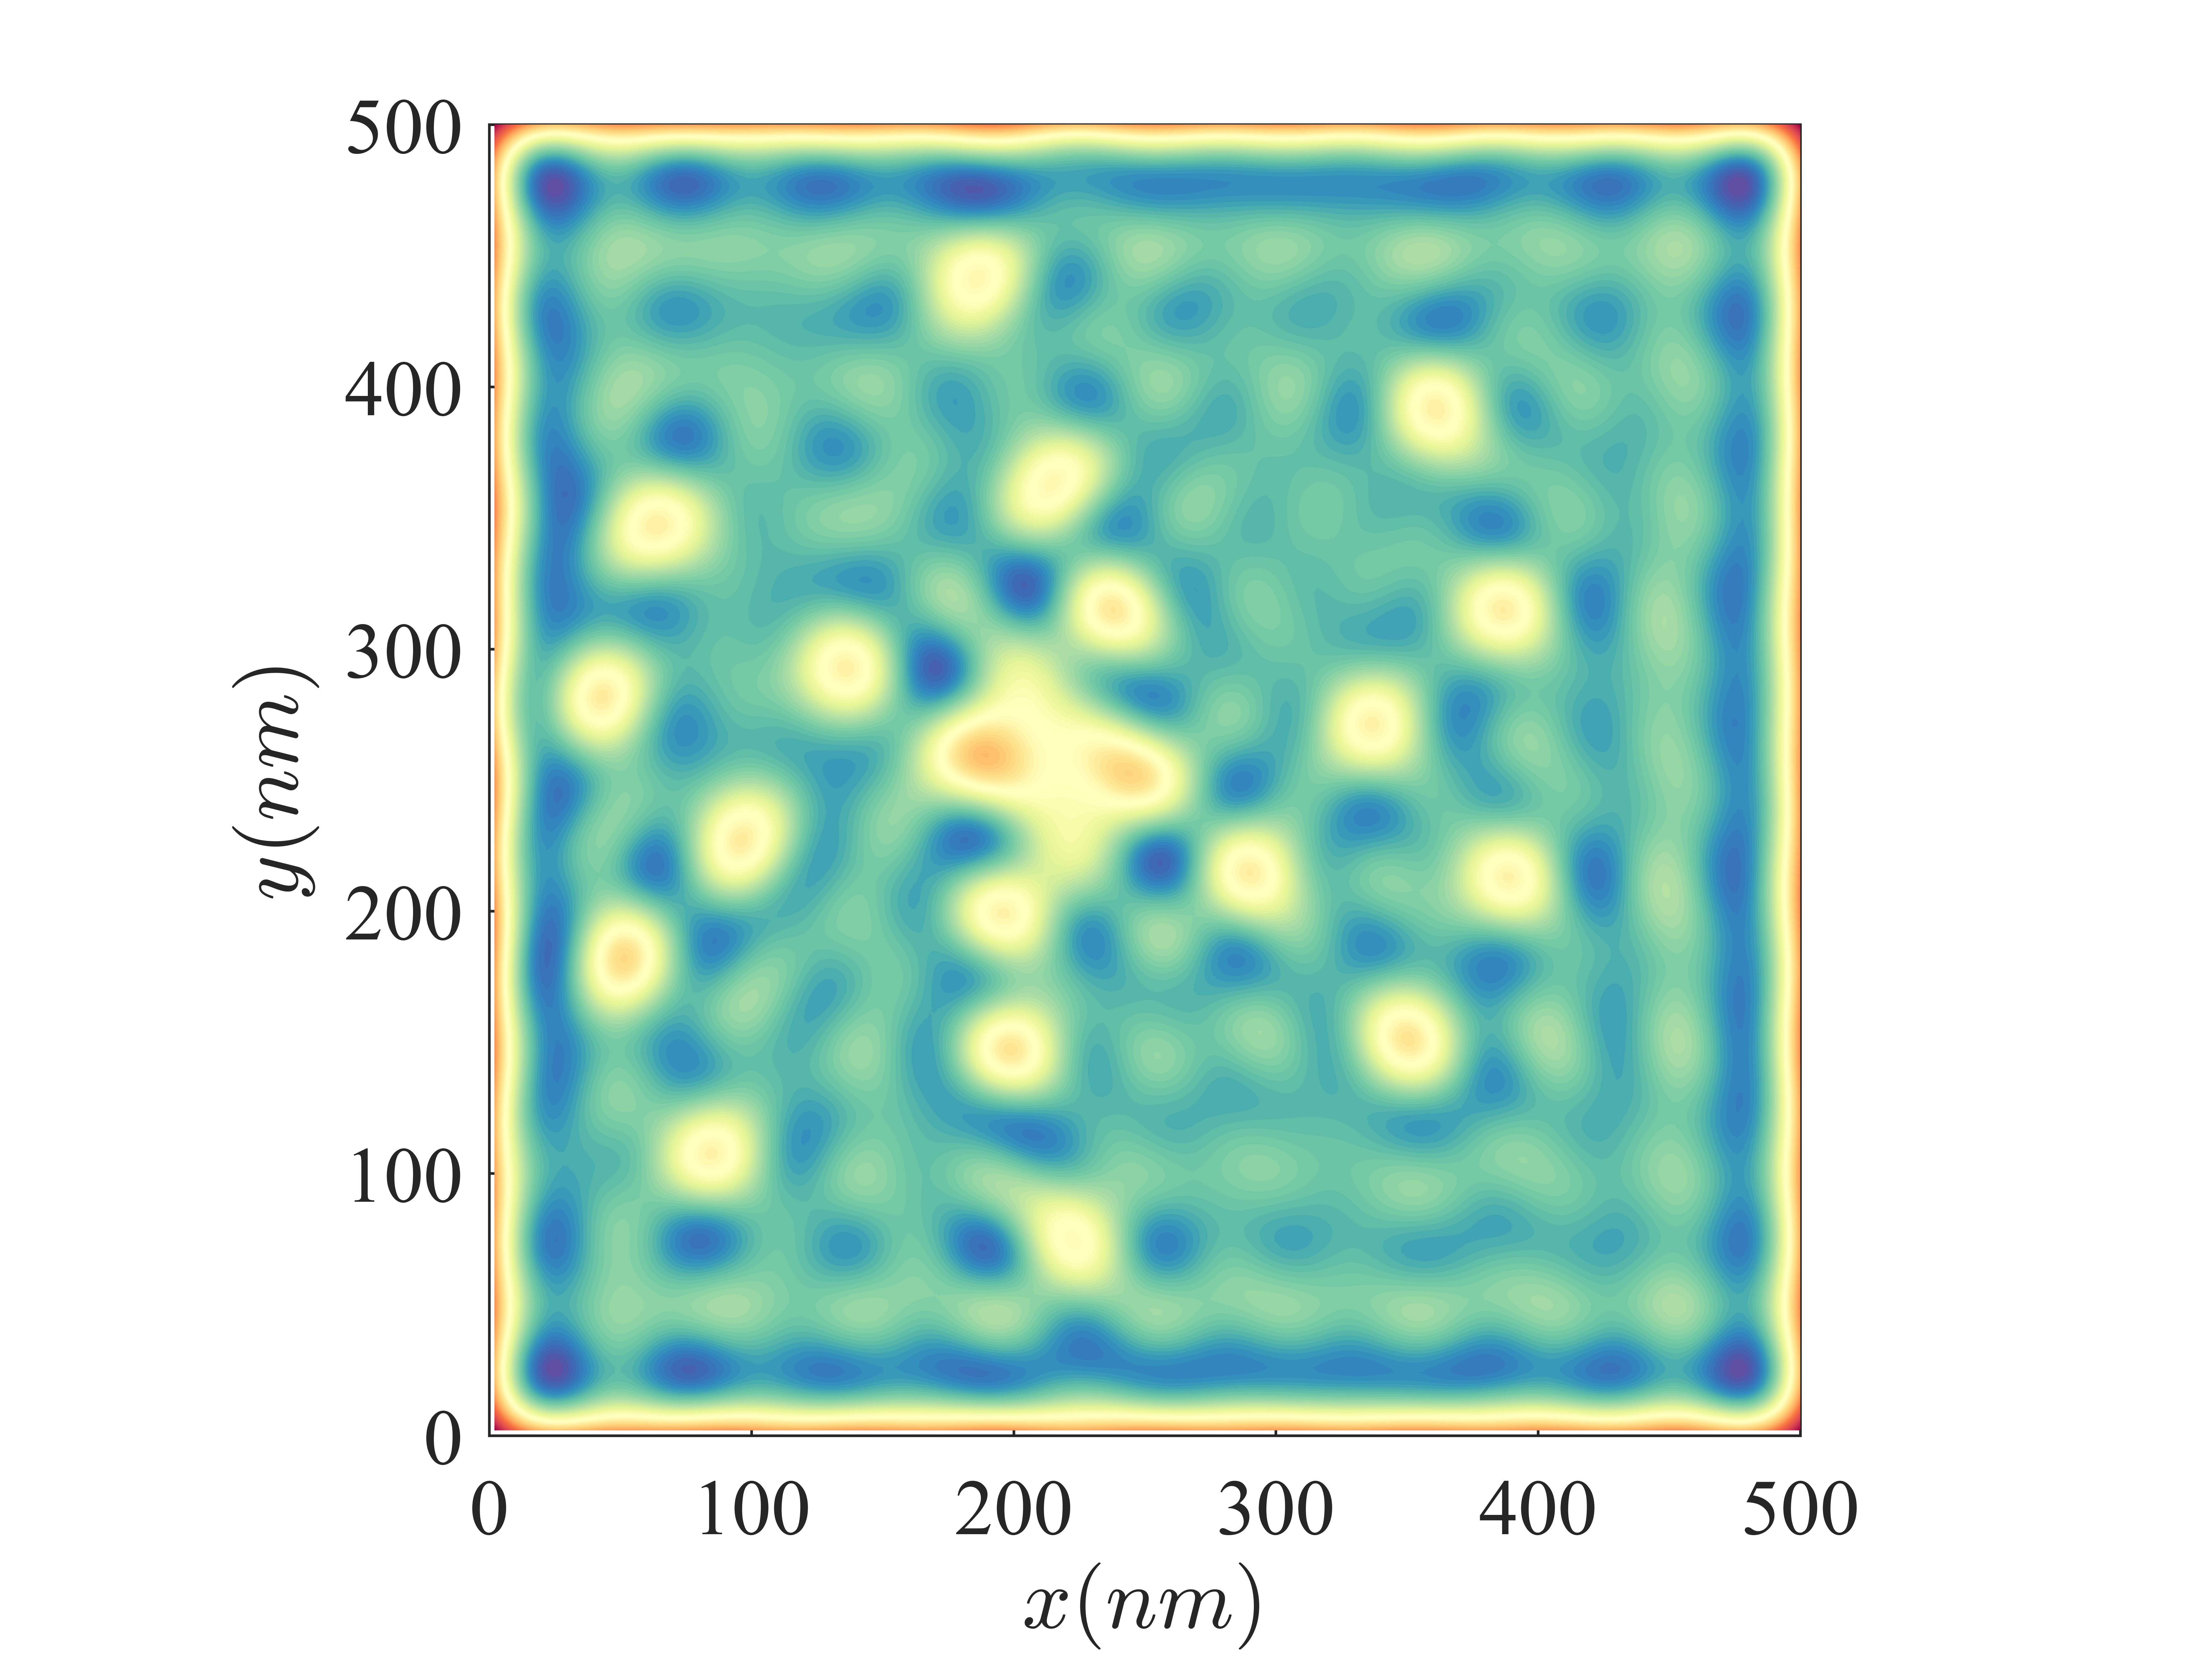
\includegraphics[scale=1]{free_space_sim.png}
  \caption{Simulation with GaAs/AlGaAs 2DEG at $20$ THz corresponding to $\Re(k_p) = 39 k_0$}
  \label{fig:sim_low}
\end{figure}

\begin{figure}[h!]
  \centering
  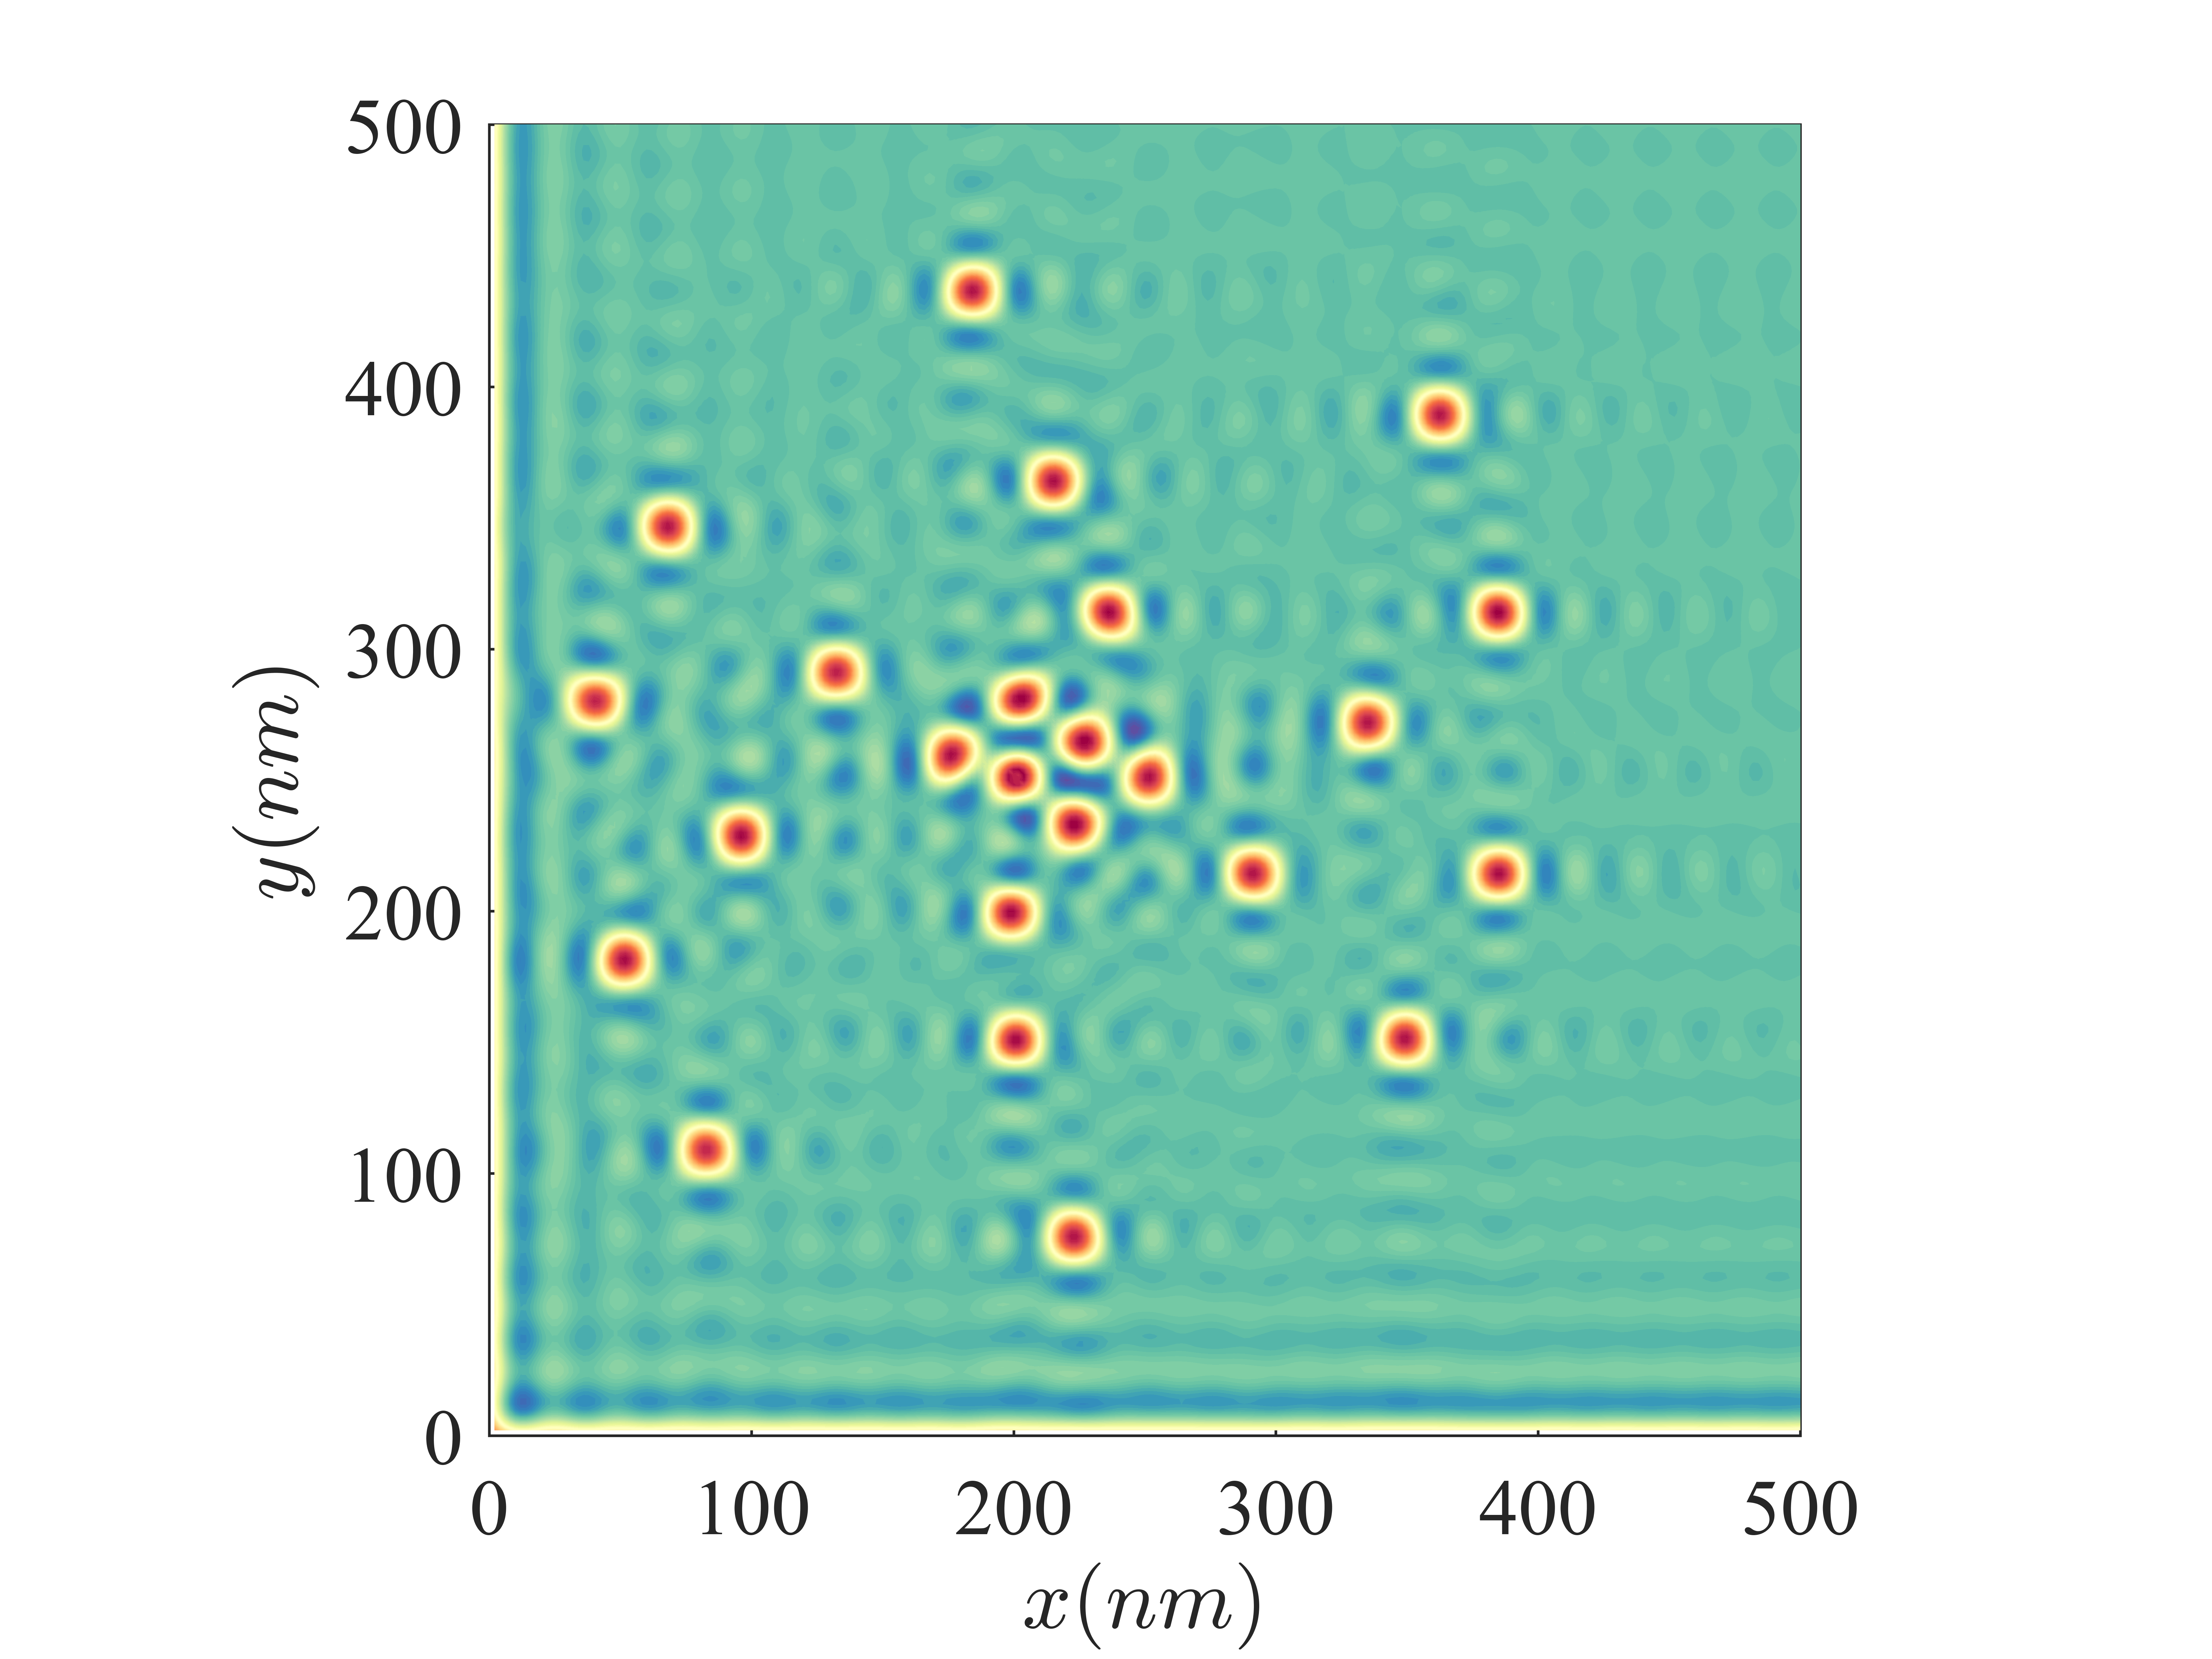
\includegraphics[scale=1]{plasmonic_sim.png}
  \caption{Simulation with GaAs/AlGaAs 2DEG at $25$ THz corresponding to $\Re(k_p) = 80 k_0$}
  \label{fig:plasmonic_sim}
\end{figure}

\clearpage % Force Bibliography to the end of document on a new page
\bibliography{zubairy}
\bibliographystyle{ieeetr}

\end{document}
